\documentclass[11pt]{article}
\usepackage[margin=1in]{geometry}
\usepackage{amsmath, amssymb, amsthm}
\usepackage{tikz}
\usetikzlibrary{arrows.meta, calc, positioning}
\usepackage{xcolor}
\usepackage{microtype}
\usepackage{hyperref}
\hypersetup{colorlinks=true, linkcolor=blue!50!black, urlcolor=blue!50!black}

\newcommand{\el}{\mathsf{el}}
\newcommand{\anc}{\mathsf{anc}}
\newcommand{\sib}{\mathsf{sib}}
\newcommand{\lo}{\mathsf{L}}
\newcommand{\ro}{\mathsf{R}}
\newcommand{\pL}{\mathsf{pL}}
\newcommand{\pR}{\mathsf{pR}}
\newcommand{\ids}{\mathsf{ids}}
\newcommand{\eff}{\mathsf{eff}}
\newcommand{\Ins}{\mathsf{Ins}}
\newcommand{\Del}{\mathsf{Del}}
\newcommand{\mrg}{\mathsf{merge}}
\newcommand{\rd}{\mathsf{read}}
\newcommand{\lca}{L}
\newcommand{\Start}{\vartriangleright}
\newcommand{\Endd}{\vartriangleleft}

\tikzset{
  vtx/.style     ={draw, circle, minimum size=8mm, inner sep=0pt, fill=blue!8, line width=0.6pt},
  sent/.style    ={draw, minimum size=6mm, inner sep=1pt, fill=black!8, font=\small},
  dead/.style    ={draw, circle, minimum size=8mm, inner sep=0pt, densely dashed, fill=black!4, text=black!40, line width=0.6pt},
  new/.style     ={draw, circle, minimum size=8mm, inner sep=0pt, fill=green!14, line width=0.7pt},
  ledge/.style   ={-{Stealth[length=2.2mm]}, line width=0.8pt},
  redge/.style   ={-{Stealth[length=2.2mm]}, line width=0.8pt, blue!55!black, densely dashed},
  capt/.style    ={font=\small\itshape, text=black!75},
  elbl/.style    ={font=\scriptsize, text=black!60},
}

\title{\bfseries The Sibling Edge\\[2pt]
\large An order-preserving, tombstone-free, RA-linearizable sequence CRDT\\[2pt]
\normalsize\itshape pen-and-paper design + Python validation (companion to \texttt{why-the-path-matters})}
\author{Sal / FP Launchpad --- KC + Claude}
\date{2026-07-13}

\begin{document}
\maketitle
\sloppy

\begin{abstract}
\noindent
The tombstone-free RGA (\texttt{RGA\_Tombstone\_Free}) converges and is
RA-linearizable, but its delete \emph{rehomes and re-sorts} survivors, so a
plain sequential delete can reorder the document ($[b,a,c]\to[c,b]$, machine-checked
as \texttt{tombstone\_free\_violates\_delete\_order}). The first ``Shesha'' fix --- a
rose-forest whose delete \emph{splices children in place} --- preserves that
order, but its three-way merge is \emph{not} a fold of any linearization
(machine-checked countermodel: $\mrg = [3,4,2]$, \texttt{Shesha\_Rows\_Refuted}):
the physical splice destroys each survivor's anchor, so the merge cannot tell a
marker's two cross-branch children apart. This note gives a third design that
has \emph{both} properties. Each element carries two \emph{immutable} origins ---
its left anchor $\lo$ (RGA's) \emph{and} a right sibling $\ro$ --- together with
their carried \emph{spine paths}. Delete simply removes the node (no rehome);
the read reconstructs the position of a deleted node from surviving neighbours'
two-sided references, and from the carried paths when a reference is one-sided.
We state the datatype, the read, and --- the point of this note --- the
\textbf{rules for merging the sibling information}, exactly parallel to how RGA
merges the anchor. A brute-force Python model then \emph{convinces us
empirically}: across $\approx$37{,}000 random merges (single- and multi-epoch)
every merge is convergent and RA-linearizable (a fold of some
$\mathsf{loOn}$-respecting linearization exists), delete-order is preserved, and
concurrent runs stay contiguous (non-interleaving). The spines are \emph{runtime
provenance} --- consulted by the read whenever a referenced origin is dead, so,
unlike RGA's proof-only carried path, they cannot be erased (\S4); the honest
boundary (the tombstoned-oracle / strong-list fooling pair remains impossible)
is unchanged. Next step: the Lean port as a conditioned instance extending
\texttt{RGA\_Tombstone\_Free}.
\end{abstract}

\section{The datatype: two immutable origins and their spines}

The state stores only \emph{live} elements. Each id $u$ (a Lamport timestamp)
records an element and \emph{two} origins:
\[
  \sigma : u \;\mapsto\; \bigl(\,\el(u),\; \lo(u),\; \ro(u),\; \pL(u),\; \pR(u)\,\bigr),
\]
where $\lo(u)$ is the element $u$ was inserted \emph{after} (its left neighbour;
$\Start$ = the start sentinel, id $0$) and $\ro(u)$ is the element it was
inserted \emph{before} (its right neighbour; $\Endd$ = the end sentinel). Both
are fixed at insert and \textbf{never mutated}. The \emph{spines} are the
ancestor chains of the two origins, recorded at insert:
\[
  \pL(u) = \bigl[\lo(u),\ \lo(\lo(u)),\ \dots,\ \Start\bigr], \qquad
  \pR(u) = \bigl[\ro(u),\ \ro(\ro(u)),\ \dots,\ \Endd\bigr].
\]
$\lo$ is exactly RGA's anchor; $\ro$ (the \emph{sibling edge}) is the addition.
Storing the right neighbour is what pins a node's position \emph{from both
sides}, so that deleting one neighbour cannot move it.

\paragraph{Read.} The document order is a linear extension of the constraints
$\{\lo(u)\prec u\prec\ro(u)\}$. Because a deleted node is gone from $\sigma$, we
\emph{reconstruct} it as a \emph{ghost}: we expand every survivor's spines into
their ghost ancestors (each carrying \emph{its} origins, read off the spine) and
integrate the whole graph, emitting only live ids.
\[
  \rd(\sigma) \;=\; \bigl[\,u \in \mathrm{topo}(G_\sigma) \ \big|\ u \in \ids(\sigma)\,\bigr],
\]
where $G_\sigma$ has an edge $g\!\to\!g'$ for every consecutive pair on a spine
($g$ the left-origin of $g'$, or $g'$ the right-origin of $g$), plus $\lo(u)\to u$
and $u\to\ro(u)$ for each live $u$. Ties (several nodes competing for one gap ---
concurrent inserts at the same origins) break \emph{newest-id-first}, the RGA
sibling rule. All origins point to \emph{older} ids, so $G_\sigma$ is acyclic and
the topological order exists and is unique.

\paragraph{The two operations.}
\begin{itemize}
  \item $\Ins(x\ \text{after}\ a)$ at fresh id $x$: read the current document,
        let $a=\lo(x)$ and $b=\ro(x)$ be $x$'s left and right neighbours there;
        store $(x,\ a,\ b,\ [a]\!:\!\pL(a),\ [b]\!:\!\pR(b))$. (Inserting at the
        front makes $a=\Start$.)
  \item $\Del(d)$: remove $d$ from $\sigma$. \textbf{Nothing else changes} --- no
        rehome, no re-sort. Survivors keep their (now possibly dead) origin ids;
        their spines still carry $d$'s origins, so the read can still place $d$'s
        ghost.
\end{itemize}

\begin{figure}[h]
\centering
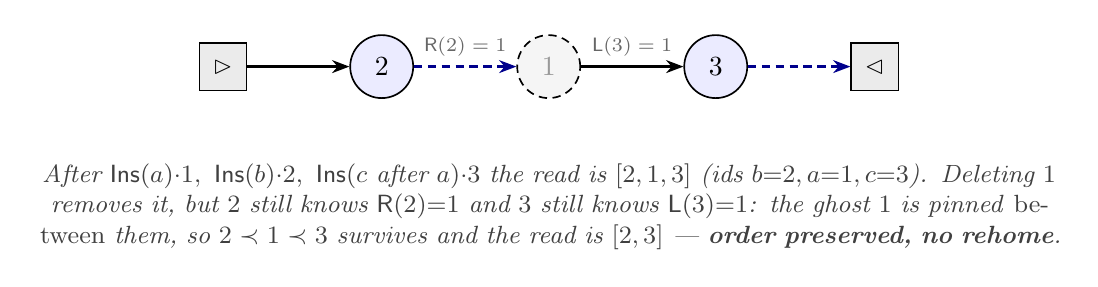
\begin{tikzpicture}[node distance=13mm]
  \node[sent] (s) {$\Start$};
  \node[vtx, right=of s] (b) {$2$};
  \node[dead, right=of b] (a) {$1$};
  \node[vtx, right=of a] (c) {$3$};
  \node[sent, right=of c] (e) {$\Endd$};
  \draw[ledge] (s) -- (b);
  \draw[redge] (b) -- (a) node[midway,above,elbl]{$\ro(2)=1$};
  \draw[ledge] (a) -- (c) node[midway,above,elbl]{$\lo(3)=1$};
  \draw[redge] (c) -- (e);
  \node[capt, text width=13cm, align=center, below=7mm of a]
    {After $\Ins(a){\cdot}1,\ \Ins(b){\cdot}2,\ \Ins(c{\ \text{after}\ }a){\cdot}3$ the read is $[2,1,3]$
     (ids $b{=}2,a{=}1,c{=}3$). Deleting $1$ removes it, but $2$ still knows
     $\ro(2){=}1$ and $3$ still knows $\lo(3){=}1$: the ghost $1$ is pinned
     \emph{between} them, so $2\prec 1\prec 3$ survives and the read is $[2,3]$ ---
     \textbf{order preserved, no rehome}.};
\end{tikzpicture}
\caption{Delete preserves order because the deleted node's position is pinned by
its two live neighbours' immutable references (the RGA design keeps only the left
one, so it must rehome and re-sort). Sibling ($\ro$) edges dashed.}
\label{fig:pin}
\end{figure}

\section{The merge --- membership, then the value rules for $\lo$ and $\ro$}

$\mrg(\lca, A, B)$ with $\lca$ the least common ancestor. As in every ternary
MRDT the survivor set is an OR-set on the three id sets,
\[
  I \;=\; \bigl(\ids\lca \cap \ids A \cap \ids B\bigr)\ \cup\
          \bigl(\ids A \setminus \ids\lca\bigr)\ \cup\
          \bigl(\ids B \setminus \ids\lca\bigr)
\]
--- an id lives unless it was in $\lca$ and deleted on a side. The \emph{values}
are where the sibling design differs from RGA, and here are the rules. Because
$\lo,\ro,\pL,\pR$ are all \textbf{immutable}, every input that stores an id
stores the \emph{same} tuple for it, so merging the fields is trivial
inheritance:
\begin{quote}
\textbf{(M1) Inherit each survivor's fields} from $\lca$ if present, else from
$A$, else from $B$ --- for \emph{both} origins and \emph{both} spines identically.
There is never a value conflict: a delete does not change any field, and inserts
are on fresh ids, so the tuple of an id is fixed for all time.
\end{quote}
This is the crux and the reason the sibling edge \emph{merges} at all: RGA has to
\emph{climb} a deleted anchor up the $\lca$ chain (\S2 of the companion note)
because its delete rehomes; here delete changes nothing, so there is nothing to
reconcile. The right origin $\ro$ is carried and inherited by exactly the same
rule as the left origin $\lo$ --- the sibling merge \emph{is} the anchor merge,
mirrored. What remains is to \emph{position} the ids in $I$:
\begin{quote}
\textbf{(M2) Order by integration over $I$ and its ghosts.} Build $G$ from the
inherited spines of the survivors (M1), \emph{including} ghost nodes for every
dead id a spine passes through --- each ghost positioned by \emph{its} carried
origins (from the spine) and by any survivor that references it. Topologically
sort (newest-id-first ties); emit the ids of $I$.
\end{quote}
\begin{quote}
\textbf{(M3) The $\lca$ does the deep remembering.} A ghost that is dead in the
merge is \emph{live in $\lca$} (it was deleted on exactly one side), so $\lca$
supplies its origins directly; a ghost dead on \emph{all} inputs is recovered
from the carried spines. Either way its position is determined --- no marker, no
splice, no rehoming.
\end{quote}
Since all origins are older ids, $G$ is acyclic and (M2) yields one deterministic
order; two replicas compute the same $I$ and the same $G$, so the merge is
convergent. \textbf{The sibling information is merged by (M1)--(M3): inherit the
right origin and its spine immutably, and let it constrain the integration
exactly as the left origin does.}

\begin{figure}[h]
\centering
\resizebox{\textwidth}{!}{%
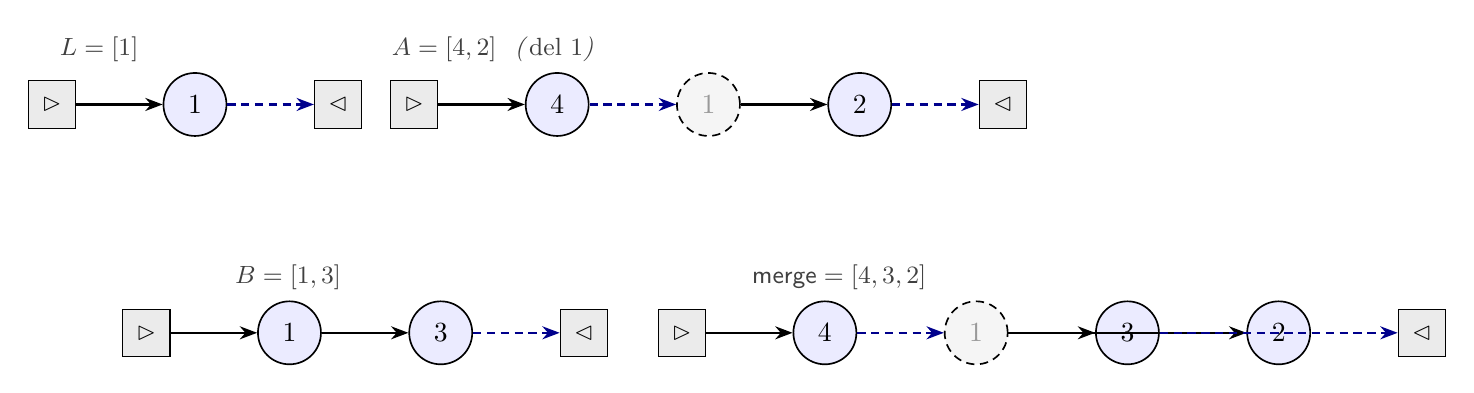
\begin{tikzpicture}[node distance=11mm]
  % LCA, A, B
  \node[capt] at (0,0.7) {$\lca=[1]$};
  \node[sent] (ls) at (-0.6,0) {$\Start$}; \node[vtx,right=of ls](l1){$1$};
  \node[sent,right=of l1](le){$\Endd$};
  \draw[ledge](ls)--(l1); \draw[redge](l1)--(le);

  \node[capt] at (5.0,0.7) {$A=[4,2]$ \ (\emph{del 1})};
  \node[sent](as) at (4.0,0){$\Start$}; \node[vtx,right=of as](a4){$4$};
  \node[dead,right=of a4](a1){$1$}; \node[vtx,right=of a1](a2){$2$};
  \node[sent,right=of a2](ae){$\Endd$};
  \draw[ledge](as)--(a4); \draw[redge](a4)--(a1); \draw[ledge](a1)--(a2); \draw[redge](a2)--(ae);

  \node[capt] at (2.4,-2.2) {$B=[1,3]$};
  \node[sent](bs) at (0.6,-2.9){$\Start$}; \node[vtx,right=of bs](b1){$1$};
  \node[vtx,right=of b1](b3){$3$}; \node[sent,right=of b3](be){$\Endd$};
  \draw[ledge](bs)--(b1); \draw[ledge](b1)--(b3); \draw[redge](b3)--(be);

  % merge
  \node[capt] at (9.4,-2.2) {$\mrg=[4,3,2]$};
  \node[sent](ms) at (7.4,-2.9){$\Start$}; \node[vtx,right=of ms](m4){$4$};
  \node[dead,right=of m4](m1){$1$}; \node[vtx,right=of m1](m3){$3$};
  \node[vtx,right=of m3](m2){$2$}; \node[sent,right=of m2](me){$\Endd$};
  \draw[ledge](ms)--(m4); \draw[redge](m4)--(m1); \draw[ledge](m1)--(m3);
  \draw[ledge](m1)--(m2); \draw[redge](m3)--(me);
\end{tikzpicture}}
\caption{The refutation countermodel, dissolved. Branch $A$ deletes marker $1$
but $4$ still carries $\ro(4)=1$ and $2$ still carries $\lo(2)=1$; branch $B$'s
$3$ carries $\lo(3)=1$. In the merge, ghost $1$ is pinned by all three: $4\prec
1\prec\{2,3\}$, ties newest-first give $3$ before $2$ --- read $[4,3,2]$, a
genuine fold. The rose-tree Shesha rehomed $2$ to the root and produced the
non-linearizable $[3,4,2]$.}
\label{fig:cx}
\end{figure}

\section{Why it is order-preserving \emph{and} linearizable}

\paragraph{Order-preserving (single replica).} $\Del(d)$ removes $d$ and
\emph{touches no other field}. The order is the linear extension of the surviving
constraints; deleting $d$ only drops $d$ from the output, never re-positions a
survivor (Figure~\ref{fig:pin}). This is the property the flat RGA refutes and
the rose-tree buys with a splice --- here it is free, because immutability plus
two-sided pinning means a survivor's neighbours (live or ghost) never change.

\paragraph{RA-linearizable.} All origins are strictly older ($\lo(u),\ro(u)<u$),
so the constraint graph is a DAG and its topological order is a total order that
extends every $\lo(u)\prec u\prec\ro(u)$. That order is exactly the naive-list
fold of \emph{some} sequential schedule of the same inserts and deletes (insert
each id between its origins, delete the dead ones), and any two orders that
disagree only on commuting operations fold to the same document. Hence the merge
read equals the read of a $\mathsf{loOn}$-respecting linearization: RA-linearizable
up to observational $=$.

\paragraph{Empirical confirmation.} \texttt{whiteboard/sibling-origin-pbt.py}
implements the datatype, the merge (M1--M3), a naive-list reference fold, and a
brute-force linearization search over $\mathsf{loOn}$ (the causal order with
\emph{commuting} pairs left unordered --- $\mathsf{rc}=\mathsf{Either}$). Over
three seeds each:
\begin{center}
\begin{tabular}{lccc}
\hline
 & merges checked & non-commutative & not-a-fold \\
\hline
single epoch ($\lca,A,B$)      & $\approx$17{,}400 & 0 & 0 \\
multi epoch (chained merges)   & $\approx$19{,}500 & 0 & 0 \\
\hline
\end{tabular}
\end{center}
Every merge converges ($\mrg(\lca,A,B)=\mrg(\lca,B,A)$, and swapped chained
merges agree) and is a fold. Hand litmus: countermodel $\to[4,3,2]$
(Fig.~\ref{fig:cx}); $[b,a,c]$ del $a\to[2,3]$ (Fig.~\ref{fig:pin}); interior
$[1,2,3]$ del $2\to[1,3]$; two concurrent runs after a common anchor stay
contiguous ($[1,20,21,10,11]$ --- non-interleaving). The multi-epoch result is
the important one: the design record feared that chained merges would break
(ghost information lost); with the carried spines, states stay self-contained and
they do not.

\section{The spines are runtime provenance --- \emph{not} ghost state; the honest boundary}

\paragraph{Corrected claim (2026-07-13; the first revision of this note wrongly
called the spines ``ghost state, as in RGA'').} RGA's carried path is ghost
state in a strict, machine-checked sense: on \emph{every reachable state} the
path is never read (\texttt{ins\_path\_free}/\texttt{del\_path\_free} --- a
client's anchor is live when it issues the op, and \texttt{resolve}
short-circuits), so a runtime implementation carries zero bytes of it; it exists
only to discharge the $\forall\sigma$-quantified commutation VC. The spines
$\pL,\pR$ are \textbf{not} that: the read consults a spine whenever a referenced
origin is dead --- which is ordinary editing, not an unreachable corner (the
\texttt{aed} trace of \S1 already uses $d$'s spine). The variant without spines
(``B2'' in the litmus suite) fails the sequential deep-delete test L3a ---
machine-checked evidence that real executions need them. So the two designs are
\emph{opposite} corners: RGA is runtime-lean with proof-only baggage; this
design carries \textbf{zero proof-only state} (application never resolves
anything, so all VCs commute without any carried certificate), and its baggage
is real runtime memory.

\paragraph{Cost, stated correctly.} A dead id persists exactly while some
\emph{live} record's birth certificate names it: the retention policy is
\emph{live-reachable ancestry}, not ``all history'' (tombstones) and not
``in-flight deletes only'' (the first revision's overstatement). Deleting a
region into which nothing live was born frees it entirely; with structural
sharing the spines are the insertion forest restricted to live-referenced
ancestry. Causal-stability compaction (rerouting spines past a stably-dead id)
is an out-of-band optimization, not part of the CRDT semantics. This memory is
not slack: the strong-list impossibility (design record \S7\textonehalf) shows
per-deletion memory is mandatory for the ordering properties this design has;
the spines are that memory, scoped by reachability.

\paragraph{What is still impossible.} Preserving order does \emph{not} recover the
tombstoned-oracle order on pairs \emph{no replica ever co-displayed}: the
$4$-node fooling pair and the $5$-node strong-list cycle (design record \S6,
\S7\textonehalf) remain impossible for any bounded tombstone-free state. Those
are strictly stronger specs than RA-linearizability; this design targets
RA-linearizability up to $=$ plus single-replica delete-order and
non-interleaving, and the licensed divergence from the tombstoned oracle is part
of the published contract, unchanged.

\paragraph{Relation to the neighbours.} Drop $\ro$ and collapse (climb) instead
of expand, and this \emph{is} \texttt{RGA\_Tombstone\_Free}: linearizable, but the
climb re-sorts and delete-order is lost. Keep $\ro$ but \emph{rehome} on delete
(mutate origins), and this is the refuted rose-tree Shesha: order-preserving, but
the mutation destroys the anchors the merge needs, so it is not a fold. The
sibling-edge design is the point between them: a second immutable origin and no
rehome.

\section{Lean port plan (conditioned instance, extending \texttt{RGA\_Tombstone\_Free})}

\begin{enumerate}
  \item State $u\mapsto(\el,\lo,\ro,\pL,\pR)$; \texttt{read} via the path-expansion
        integration; \texttt{insert}/\texttt{delete} as above. Sequential soundness:
        \texttt{read} $=$ the naive list (mirror \texttt{RGA\_Tombstone\_Free\_ReadSide}).
  \item \texttt{merge} $=$ (M1) inherit $+$ (M2) integrate; \texttt{merge\_comm}
        (symmetry) and well-formedness (acyclicity from id-monotone origins).
  \item Order-preservation: \texttt{delete\_preserves\_survivor\_order} as a
        \emph{sequential} theorem (contrast the flat RGA's refutation) --- now
        \emph{true}, unlike the rose-tree at the merge level.
  \item Single-replica commutation: application is record add/remove and never
        resolves a reference, so \emph{all} operation pairs commute at the state
        level --- no accuracy conditioning, no carried proof-only certificate;
        the flat VC engine should apply (the OR-set route). Spine
        \emph{validity} (each spine is the genuine birth ancestry) is an
        invariant consumed by the ReadSide intent theorems, not by convergence.
  \item RA-linearizability capstone \texttt{sib\_ra\_linearizable3\_eq} via the
        LCA-climb join, reusing \texttt{RGA\_Tombstone\_Free}'s honest-delivery
        scaffolding: the merge is the linearization witness (integration order).
\end{enumerate}
The Python model (\S4) is the executable specification the Lean \texttt{read} and
\texttt{merge} must match, and the litmus/countermodel cases are the SPOTs.

\end{document}
